<USER_REQUEST>
%==============================================================================
%  IEEE JOURNAL PAPER  --  Overleaf-ready, self-contained (no external .bib)
%  Project: arxml-secdiff   (REVISION 2: corrected against a re-run of the code)
%
%  HOW TO USE
%    1. New Overleaf project, upload THIS FILE ONLY (main.tex).
%    2. Menu -> Compiler -> pdfLaTeX. Compile twice (cross-references).
%    3. Everything (diagrams, charts, tables) is drawn in-line.
%
%  WHAT CHANGED IN THIS REVISION (all verified by running the repository):
%    * Case study rewritten. Running each change of scenario B ALONE shows that
%      BOTH single changes already BLOCK, so the "two benign changes compose"
%      claim and the "adding gwToAdas alone would only reach adas at risk 3"
%      counterfactual were removed everywhere (abstract, intro, case study,
%      conclusion). A new table reports the three runs.
%    * Scoring section corrected (assumed-marking rule, fixed-impact
%      categories, impact-resolution order, feasibility behaviour).
%    * Scope sentence on SecOC removal corrected (no route is required).
%    * Gate: inconclusive_blocks option documented.
%    * Line count split into tool vs. evaluation harness.
%    * Abstract now states the flag-based recall next to the label-based score.
%    * Limitations extended (syntactic benign corpus, scoring choices, rename
%      masking, informational share of "regressions").
%    * Linux re-run timings added; unverified figures softened.
%
%  Items marked  % VERIFY  or shown in red as [cite]  still need YOUR input
%  (real citations, venue, department).  Nothing in the numbers is guessed.
%==============================================================================

\documentclass[journal]{IEEEtran}
\IEEEoverridecommandlockouts

%------------------------------- PACKAGES -------------------------------------
\usepackage{cite}
\usepackage{amsmath,amssymb,amsfonts}
\usepackage{algorithm}
\usepackage{algpseudocode}
\usepackage{graphicx}
\usepackage{xcolor}
\usepackage{booktabs}
\usepackage{array}
\usepackage{tikz}
\usetikzlibrary{shapes.geometric, arrows.meta, positioning, fit, backgrounds, calc}
\usepackage{pgfplots}
\pgfplotsset{compat=1.18}
\usepackage{url}
\usepackage[hidelinks]{hyperref}

\newcommand{\needcite}{\textcolor{red}{[cite]}}

\begin{document}

%---------------------------------- TITLE -------------------------------------
\title{Continuous Security Validation for Connected Vehicle Software Using a Graph-Based Approach to Detect Attack Paths in Over-the-Air Updates}

\author{%
\begin{tabular}{@{}c@{\hspace{1.6em}}c@{\hspace{1.6em}}c@{}}
\textit{Dr.~Nagasundari~S} & \textit{Kushal~D} & \textit{Manamohan~C~A}\\
PES University & PES University & PES University\\
Bengaluru, India & Bengaluru, India & Bengaluru, India\\
\textit{nagasundaris@pes.edu} & \textit{1811kushald@gmail.com} & \textit{manmohanca42005@gmail.com}\\[1.2ex]
\end{tabular}\\[0.5ex]
\begin{tabular}{@{}c@{\hspace{1.6em}}c@{}}
\textit{Purushotham} & \textit{Hithaishi~Gowda}\\
PES University & PES University\\
Bengaluru, India & Bengaluru, India\\
\textit{purushothamgowda2005@gmail.com} & \textit{hithutgowda@gmail.com}\\
\end{tabular}%
\thanks{Manuscript submitted September 2026.}%
\thanks{The authors are with PES University, Bengaluru, India
(e-mail: nagasundaris@pes.edu; 1811kushald@gmail.com;
manmohanca42005@gmail.com; purushothamgowda2005@gmail.com;
hithutgowda@gmail.com).}}  % VERIFY: add department / correct affiliation line

\markboth{IEEE Transactions on X, Vol.~XX, No.~X, 2026}% VERIFY: real venue
{Author \MakeLowercase{\textit{et al.}}: Reachability-Aware Detection of Security Regressions Between AUTOSAR ARXML Snapshots}

\maketitle

%--------------------------------- ABSTRACT -----------------------------------
\begin{abstract}
Software-defined vehicles are updated frequently over-the-air (OTA), and each update rewrites the AUTOSAR architecture that specifies how in-vehicle software components interact. A change that appears innocuous in a syntactic diff can nonetheless introduce a catastrophic security regression, because automotive security depends not on individual XML lines, but on whether an untrusted external interface can reach and influence safety-critical actuators along an unauthenticated path. We present \textsc{arxml-secdiff}, an automated release-gate tool that analyzes differences between two AUTOSAR ARXML snapshots to detect newly created or modified attack paths. The tool constructs a prototype-keyed influence graph with two-edge client--server semantics; evaluates Secure Onboard Communication (SecOC) using a three-valued logic distinguishing unauthenticated bus hops from secure local runtimes; computes newly reachable entry-to-critical paths; scores findings via an ISO/SAE~21434-aligned risk matrix with downstream severity inheritance; and renders an auditable four-verdict gate (\textsc{Pass}, \textsc{Flag}, \textsc{Block}, \textsc{Inconclusive}) integrated with continuous integration (CI/CD) pipelines. We evaluate the tool across four detection paradigms over a benchmark of thirteen real-world vehicle exploit and boundary scenarios, an alert fatigue test of 93 benign refactoring commits, and an expanded multi-site mutation corpus. Across all 93 benign commits, \textsc{arxml-secdiff} achieves a $0.0\%$ false alarm rate (100\% noise elimination), compared to false alarm rates of $84.9\%$ to $98.9\%$ for textual and structural diff baselines. Under camouflaged multi-site attack compositions, we demonstrate an empirical precision decay curve (finding precision degrades from $97.3\%$ to $75.0\%$ from Order~1 to Order~4 as alert dispersion occurs) while maintaining strict release-blocking capability. Analysis latency averages $6.57$~ms (median $6.30$~ms) with $\mathcal{O}(V+E)$ linear complexity, enabling sub-10ms automated pre-commit gating. Finally, we formulate a formal taxonomy of four architectural failure modes, establishing the boundary between structural model differencing and low-level firmware execution.
\end{abstract}

\begin{IEEEkeywords}
AUTOSAR, ARXML, automotive security, security regression, SecOC, attack-path
reachability, ISO/SAE~21434, release gate, CI/CD, threat modeling.
\end{IEEEkeywords}

\IEEEpeerreviewmaketitle

%================================ 1. INTRODUCTION =============================
\section{Introduction}
\label{sec:intro}

\IEEEPARstart{M}{odern} vehicles are defined by software. A single car
integrates hundreds of software components communicating across several
electronic control units (ECUs) and in-vehicle buses, and the whole assembly
is described by the AUTOSAR standard~\cite{autosar} as a set of XML documents
in the ARXML (AUTOSAR XML) format. As over-the-air (OTA) updates become
routine, this architecture no longer changes once at design time; it changes
every release, and regulation now expects manufacturers to manage cybersecurity
across the vehicle lifecycle~\cite{unr155,iso21434}. Each release therefore
reopens a question that safety and security engineering would prefer to settle
once: does the new architecture let an attacker reach something dangerous that
the previous architecture protected? Published remote compromises of
production vehicles~\cite{koscher,checkoway,miller} share this structure: an
attacker-reachable interface, a missing authentication hop, and a route to a
safety-critical function.

The natural first instinct---compare the two ARXML files with a diff tool---is
inadequate, and understanding \emph{why} it is inadequate motivates the whole
design of this work. A textual or XML diff answers ``which elements changed,''
but security is not a property of individual elements. It is a property of
\emph{paths}: whether an exposed interface can influence a critical actuator,
and whether the messages along the way are authenticated. Three consequences
follow. First, a diff is noisy: reordering sibling elements, renaming a
connector, or reformatting whitespace all register as changes although none
alters behaviour. Second, a diff is blind to danger: adding a connector between
two comfort components and adding a connector that bridges the infotainment
domain to the braking domain look identical at the XML level. Third, and most
importantly, a diff cannot see \emph{consequence along a path}: a single new
connector can join hops that already exist and so complete an end-to-end route
from an attacker's entry point to a safety-critical target, yet the changed
lines say nothing about the hops it connects to. A reviewer reading a flat list
of changed lines has no way to notice that the new edge completes a route.

\subsection{Problem Statement}
\label{subsec:problem}

We address the following problem. Given two AUTOSAR ARXML snapshots---the
architecture before an update and the architecture after it---together with a
declaration of which components are attacker entry points and which are
safety-critical, decide automatically whether the update introduces a security
regression, and do so with a verdict precise enough to gate a release in an
automated pipeline. The decision must be low-noise, because a gate that cries
wolf on every rename is switched off; it must be honest, because a gate that
reports a clean pass when it never actually analysed anything is worse than no
gate; and it must be explainable, because a blocked release must come with the
exact route and the exact unauthenticated hop that justify the block.

\subsection{Threat Model and Scope}
\label{subsec:scope}

We consider an attacker who controls a vehicle interface that is exposed by
design---for example a Bluetooth or Wi-Fi stack, a USB or diagnostic entry, or
a remotely reachable telematics/infotainment component---and who seeks to
influence a safety-critical function such as a braking or steering actuator.
The assets are the components an organization's hazard and risk analysis
(HARA) and threat analysis and risk assessment (TARA) mark as safety-critical,
carried in this work as ASIL-rated roles. The analysis is performed at the
architectural level: it reasons about which component can influence which, and
about whether in-vehicle messages are authenticated with SecOC, but it does not
reason about source-code defects, timing side channels, or physical tampering,
which are out of scope.

Within this model the tool targets a fixed, enumerable set of regression
classes, each of which corresponds to a concrete finding category
(Section~\ref{subsec:findings}). The headline class is a \emph{newly reachable
critical node}: an entry point that can influence a safety-critical component
that it provably could not influence before. The remaining classes are the
architectural moves that create or aggravate such reachability or exposure:
removal of SecOC authentication from a bus-visible message (\emph{SecOC
removal}), which the scorer rates against the safety-critical target the
message feeds whether or not an attacker route to it currently exists
(Section~\ref{subsec:severity}); placing a previously RTE-internal signal onto a
bus without authentication (\emph{unprotected new hop} and \emph{newly
bus-visible}); and relocating a component across an ECU boundary so that
traffic newly traverses a bus (\emph{component rehosting}). Adding, removing and
rehosting components are reported but are \emph{informational}: by design they
cannot by themselves change the verdict.

\subsection{Contributions}
\label{subsec:contrib}

This paper makes the following contributions, each of which is realized in a
working, tested implementation of about $7{,}460$ lines across $22$ Python
modules (about $4{,}500$ lines of analysis code and about $2{,}900$ lines of
mutation and evaluation harness) with $401$ tests.

\begin{enumerate}
\item A \emph{prototype-keyed influence graph} that models an AUTOSAR
architecture for security reachability. Nodes are component \emph{prototypes}
(instances), not types, so that two instances of one component remain distinct;
and a client--server connector is modelled as \emph{two} directed edges
(request and response) so that the direction an attacker actually travels is
never lost (Section~\ref{sec:design}).

\item A \emph{three-valued SecOC analysis} that distinguishes ``authentication
does not apply here'' (an RTE-internal connector) from ``authentication applies
and is missing'' from ``authentication is present.'' Collapsing the first into
the second would label every RTE-local connector as unprotected; keeping them
apart is the design choice intended to let the gate stay quiet on benign
changes (Section~\ref{subsec:secoc}). We do not report an ablation against a
boolean model; see Section~\ref{sec:discussion}.

\item \emph{Reachability differencing} that computes attacker-to-critical paths
on both snapshots and reports only pairs that are \emph{newly} reachable, each
annotated with the authentication state of every hop along the route
(Section~\ref{subsec:reach}).

\item \emph{Provenance-aware risk scoring and an auditable four-verdict gate}.
Findings are scored on an ISO/SAE~21434-style matrix; hop findings can inherit
impact from the worst safety-critical target downstream; findings built on
\emph{guessed} inputs are marked and can only flag, never block; and the gate
emits \textsc{Pass}/\textsc{Flag}/\textsc{Block}/\textsc{Inconclusive} with CI
exit codes, refusing to award a clean pass to an analysis that never ran
(Sections~\ref{subsec:severity}--\ref{subsec:gate}).

\item An \emph{extensive empirical evaluation across four detection paradigms} spanning thirteen real-world exploit and boundary replay scenarios, an industrial noise study of $93$ benign commits, and a multi-site mutation corpus of $285$ cases. We show $100\%$ noise elimination ($0.0\%$ false-positive rate) on benign edits, characterize the empirical precision decay curve ($97.3\%$ to $75.0\%$) under multi-site camouflage, validate sub-10ms operational gating latency ($6.30$~ms median), and articulate a taxonomy of four concrete architectural failure modes (Sections~\ref{sec:eval} and~\ref{sec:results}).
\end{enumerate}

\subsection{Paper Organization}
Section~\ref{sec:background} gives the AUTOSAR and ISO/SAE~21434 background.
Section~\ref{sec:related} positions the work against prior approaches.
Section~\ref{sec:design} presents the system design and data model.
Section~\ref{sec:impl} details the algorithms, scoring, and gate.
Section~\ref{sec:eval} describes the simulation and evaluation harness.
Section~\ref{sec:results} reports results, including the flagship case study.
Section~\ref{sec:discussion} discusses limitations, and
Section~\ref{sec:conclusion} concludes.

%============================== 2. BACKGROUND ================================
\section{Background}
\label{sec:background}

\subsection{AUTOSAR and the ARXML Format}
AUTOSAR describes a vehicle's software architecture as software-component types,
the ports through which they communicate, the interfaces those ports realize,
and the connectors that wire ports together, all serialized as ARXML. A
component \emph{type} may be instantiated many times; each instance is a
\emph{prototype} with its own path. Communication is either sender--receiver
(data flow) or client--server (request/response invocation). A composition
component groups instances and connects them, and \emph{delegation} connectors
expose an inner port at the boundary of a composition. Physically, components
are mapped onto ECU instances, and signals that cross ECUs are packed into
I-signal I-PDUs carried on a bus. The same logical model is emitted under two
schema revisions (R3 and R4) that differ only in their XML namespace URI, so a
robust reader must be namespace-agnostic.

\subsection{Secure Onboard Communication (SecOC)}
SecOC authenticates selected in-vehicle PDUs by wrapping a payload PDU in a
\texttt{SECURED-I-PDU} that carries a message authentication code and freshness
value. Authentication is therefore a property of a \emph{PDU on a bus}, not of a
logical connector: a connector whose signals never leave an ECU has no PDU to
protect, and asking whether it is ``authenticated'' is a category error. This
distinction is the technical basis for the three-valued analysis in
Section~\ref{subsec:secoc}.

\subsection{ISO/SAE~21434 Risk}
ISO/SAE~21434~\cite{iso21434} frames automotive cybersecurity risk as a
combination of \emph{impact} (how bad is the damage) and \emph{attack
feasibility} (how easy is the attack), combined through a risk matrix into a
value on a small ordinal scale. We adopt this framing directly: impact is driven
by the ASIL of the safety-critical asset a finding endangers, feasibility is
driven by whether the route crosses a bus unauthenticated and whether its entry
point is remotely accessible, and the two are combined by the matrix of
Table~\ref{tab:riskmatrix}.

%============================== 3. RELATED WORK =============================
\section{Related Work}
\label{sec:related}

% VERIFY all citations below (fogel, ou) against the original sources.
Prior work relevant to this problem falls into five groups. Experimental
studies of production vehicles~\cite{koscher,checkoway,miller} and surveys of
attacks on automated vehicles~\cite{petit} establish the attack structure that
motivates this work, but they study vehicles and exploits rather than
release-to-release architecture change. Model- and architecture-level
automotive security analysis reasons about a vehicle model to surface
security-relevant structure, but typically analyses a single model rather than
the \emph{difference} between two releases, which is the quantity a release gate
must judge \needcite. Work on SecOC and in-vehicle authentication studies the
mechanism itself and its configuration, generally treating the presence of
authentication as a boolean rather than distinguishing the case in which
authentication is not applicable at all \needcite. Attack-graph and
reachability analysis~\cite{sheyner,ou}, including the TARA methods encouraged
by ISO/SAE~21434, models paths from entry points to assets, but is usually
applied as a design-time exercise rather than wired into a per-commit gate with
an auditable verdict. Differential reachability checking is established in
network-configuration verification~\cite{fogel}, where two configurations are
compared by the reachability they permit; we apply the same idea to AUTOSAR
architectures, where the domain-specific parts are the prototype-level graph,
the SecOC semantics and the ISO/SAE~21434-style gate. Finally, textual and
structural differencing, including fine-grained change extraction on structured
artifacts~\cite{fluri}, is the standard tool for detecting change in
configuration management, but---as Section~\ref{sec:intro} argued and
Section~\ref{sec:results} measures---it detects change without any notion of
security danger or of consequence along a path. We evaluate with
mutation-generated labelled pairs, following the mutation-testing
tradition~\cite{jia}.

Table~\ref{tab:related} summarizes the distinction (``Diff'' = compares two
releases; ``3-val.'' = three-valued SecOC). The contribution is the combination,
for AUTOSAR ARXML, of prototype-level reachability differencing, three-valued
SecOC reasoning, provenance-aware risk scoring, and an auditable, CI-ready
release verdict with measured false-positive control.
% NOTE: rows marked [cite] must be completed from a systematic literature
% search before submission; the novelty claim is only as strong as that search.

\begin{table}[t]
\centering
\caption{Positioning Against Categories of Prior Work.}
\label{tab:related}
\renewcommand{\arraystretch}{1.25}
\footnotesize
\setlength{\tabcolsep}{3pt}
\begin{tabular}{@{}p{2.3cm}ccccc@{}}
\toprule
\textbf{Approach} & \textbf{Graph} & \textbf{Reach.} & \textbf{Diff} & \textbf{3-val.} & \textbf{Gate} \\
\midrule
Model-level analysis \needcite   & \checkmark & --         & --         & --      & -- \\
SecOC config.\ \needcite         & --         & --         & --         & partial & -- \\
Attack graphs \cite{sheyner,ou}  & \checkmark & \checkmark & --         & --      & -- \\
Network diff.\ reach.\ \cite{fogel} & \checkmark & \checkmark & \checkmark & --   & -- \\
Tree/text diff \cite{fluri}      & --         & --         & \checkmark & --      & -- \\
\midrule
\textbf{This work} & \checkmark & \checkmark & \checkmark & \checkmark & \checkmark \\
\bottomrule
\end{tabular}
\end{table}

%============================== 4. SYSTEM DESIGN =============================
\section{System Design}
\label{sec:design}

\subsection{Pipeline Overview}
The tool is a linear pipeline (Fig.~\ref{fig:pipeline}). Two ARXML snapshots are
parsed into a common model; each is turned into an influence graph; each graph
is annotated with SecOC status; entry and critical roles are classified
(from a configuration file, or heuristically when none is given); reachability
is computed on each snapshot; the two graphs are structurally differenced
(together with the SecOC profile sets) and the two reachability results are
differenced; the resulting findings are scored; and the scored findings are
passed through the release gate, which returns a verdict and a process exit
code. Every stage is namespace-agnostic and side-effect free, so the same inputs
always produce the same verdict.

\begin{figure}[t]
\centering
\resizebox{\columnwidth}{!}{%
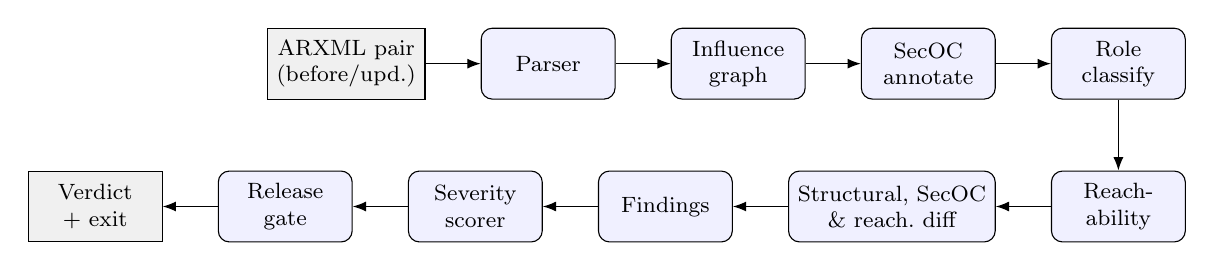
\begin{tikzpicture}[
  font=\footnotesize, >=Latex, node distance=6mm and 7mm,
  stage/.style={draw, rounded corners, minimum height=9mm, minimum width=17mm, align=center, fill=blue!6},
  io/.style={draw, minimum height=9mm, minimum width=17mm, align=center, fill=black!6}
]
  \node[io] (in) {ARXML pair\\(before/upd.)};
  \node[stage, right=of in] (parse) {Parser};
  \node[stage, right=of parse] (graph) {Influence\\graph};
  \node[stage, right=of graph] (secoc) {SecOC\\annotate};
  \node[stage, right=of secoc] (roles) {Role\\classify};
  \node[stage, below=9mm of roles] (reach) {Reach-\\ability};
  \node[stage, left=of reach] (diff) {Structural, SecOC\\\& reach.\ diff};
  \node[stage, left=of diff] (find) {Findings};
  \node[stage, left=of find] (score) {Severity\\scorer};
  \node[stage, left=of score] (gate) {Release\\gate};
  \node[io, left=of gate] (out) {Verdict\\+ exit};
  \draw[->] (in)--(parse);
  \draw[->] (parse)--(graph);
  \draw[->] (graph)--(secoc);
  \draw[->] (secoc)--(roles);
  \draw[->] (roles)--(reach);
  \draw[->] (reach)--(diff);
  \draw[->] (diff)--(find);
  \draw[->] (find)--(score);
  \draw[->] (score)--(gate);
  \draw[->] (gate)--(out);
\end{tikzpicture}}
\caption{The \textsc{arxml-secdiff} pipeline. Two snapshots are parsed, turned
into SecOC-annotated influence graphs, role-classified and searched for
attacker reachability; the graphs, SecOC profiles and reachability results are
differenced, and the findings are scored and gated into a verdict with a CI exit
code.}
\label{fig:pipeline}
\end{figure}

\subsection{The Influence Graph}
\label{subsec:graph}
The core data structure is a directed multigraph whose nodes are component
\emph{prototypes} and whose edges are the connectors between their ports. Two
design decisions distinguish it from a naive component-type graph.

\emph{Prototype keying.} A node is keyed on the prototype path, not the
component type. If a door-control type is instantiated as a left and a right
door, the graph holds two nodes, so a change that affects only one instance is
localized to it. Each node records its provided and required ports, its
enclosing composition, and its host ECU (or \texttt{None} when the snapshot
declares no SWC-to-ECU mapping).

\emph{Client--server yields two edges.} A sender--receiver connector produces a
single data edge from provider to requester. A client--server connector,
however, produces \emph{two} edges: a request edge from requester to provider
and a response edge from provider back to requester (Fig.~\ref{fig:cs}). This
matters for reachability: an attacker who controls a client can influence the
server through the request direction, and modelling only the provider-to-user
direction would silently lose exactly the edge the attacker travels. Parallel
connectors are preserved as parallel edges (the graph is a multigraph), so no
two physical connectors are ever conflated. Assembly edges additionally record
whether they cross an ECU boundary---\texttt{True} on a bus, \texttt{False}
RTE-local, \texttt{None} when an endpoint is unmapped---and delegation
connectors are represented with explicit inward/outward direction.

\begin{figure}[t]
\centering
\resizebox{0.85\columnwidth}{!}{%
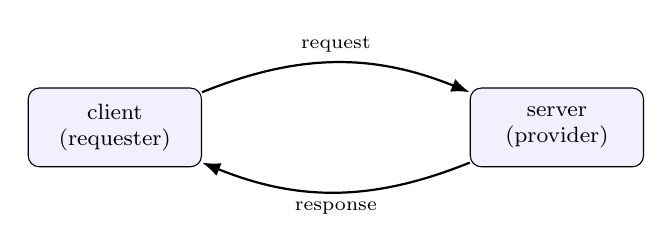
\begin{tikzpicture}[
  font=\footnotesize, >=Latex,
  comp/.style={draw, rounded corners, minimum height=10mm, minimum width=22mm, align=center, fill=blue!6}
]
  \node[comp] (c) {client\\(requester)};
  \node[comp, right=34mm of c] (s) {server\\(provider)};
  \draw[->, thick] (c) to[bend left=22] node[above,font=\scriptsize]{request} (s);
  \draw[->, thick] (s) to[bend left=22] node[below,font=\scriptsize]{response} (c);
\end{tikzpicture}}
\caption{One client--server connector becomes two directed edges. The request
edge is the direction an attacker controlling the client travels toward the
server, and is the edge a provider-to-user model loses.}
\label{fig:cs}
\end{figure}

\subsection{Formal Definitions}
Let each snapshot induce an influence graph $G=(V,E)$, where $V$ is the set of
component prototypes and $E$ the set of connector edges, each edge carrying an
authentication label $a(e)\in\{\textsc{None},\textsc{False},\textsc{True}\}$ and
a bus-visibility flag. Let $S\subseteq V$ be the attacker entry points and
$C\subseteq V$ the safety-critical targets. A target $c\in C$ is
\emph{reachable} from an entry $s\in S$ if there is a simple directed path
$s\rightsquigarrow c$ in $G$ of length at most a cutoff $k$ (counted in edges).
Writing $\mathrm{Pairs}(G)=\{(s,c): s\in S,\, c\in C,\, s\rightsquigarrow c\}$,
the \emph{newly reachable} set for a before/updated pair $(G_b,G_u)$ is
$\mathrm{Pairs}(G_u)\setminus\mathrm{Pairs}(G_b)$. Reachability depends only on
the topology of $G$; the labels $a(e)$ enter later, through feasibility. Each
finding $f$ is scored by
\begin{equation}
\label{eq:risk}
r(f)=M\big(\mathrm{impact}(f),\,\mathrm{feasibility}(f)\big),\qquad r\in\{1,\dots,5\},
\end{equation}
where $M$ is the risk matrix of Table~\ref{tab:riskmatrix}.

%============================== 5. IMPLEMENTATION ============================
\section{Implementation}
\label{sec:impl}

The tool is implemented in Python ($\geq 3.10$) in $22$ modules totalling about
$7{,}460$ lines, of which about $4{,}500$ are the analysis itself and about
$2{,}900$ are the mutation generator and evaluation harness. It depends at run
time on \texttt{lxml} for XML, \texttt{networkx} for the graph,
\texttt{PyYAML} for role and policy configuration, and \texttt{matplotlib} (with
\texttt{seaborn} for the evaluation figures) for rendering; \texttt{pytest} is
needed only for the test suite. It installs as the console command
\texttt{arxml-secdiff}. Parsing is deliberately namespace-agnostic: the reader
matches on the XML \emph{local name} of each element, so the same code handles
both the R3 and R4 schema revisions, which differ only in namespace URI.

\subsection{Core Analysis Algorithm}
Algorithm~\ref{alg:main} is the top-level analysis. It is written as a sequence
of explicit stages, mirroring the pipeline, so that every intermediate---the two
graphs, the structural diff, the two reachability results---is available to the
gate for the honesty checks described below. The same role configuration is
applied to both snapshots; using different seeds on either side would make the
reachability difference meaningless.

\begin{algorithm}[t]
\caption{Security-Regression Analysis}
\label{alg:main}
\begin{algorithmic}[1]
\Require ARXML snapshots $A_{b},A_{u}$; roles $R$ (or heuristics); policy $P$
\Ensure Verdict $v\in\{\textsc{Pass},\textsc{Flag},\textsc{Block},\textsc{Inconclusive}\}$ and exit code
\ForAll{$X \in \{b,u\}$}
  \State $M_X \gets \Call{Parse}{A_X}$;\ \ $G_X \gets \Call{BuildGraph}{M_X}$
  \State $\Call{AnnotateSecOC}{G_X, M_X}$
  \State $R_X \gets \Call{Classify}{G_X, R}$;\ \ $r_X \gets \Call{Reach}{G_X,R_X}$
\EndFor
\State $D \gets \Call{Diff}{G_b,G_u}$ \Comment{nodes, edges, SecOC profiles}
\State $RD \gets \Call{ReachDiff}{r_b,r_u}$ \Comment{newly reachable pairs}
\State $F \gets \Call{CollectFindings}{D,\,RD}$
\ForAll{$f \in F$}
  \State $f.\mathit{score} \gets \Call{Score}{f,\,R_u,\,r_u}$ \Comment{Eq.~\eqref{eq:risk}}
\EndFor
\State \Return $\Call{Gate}{F,\,P}$
\end{algorithmic}
\end{algorithm}

\subsection{Three-Valued SecOC Annotation}
\label{subsec:secoc}
For each connector edge the annotator collects the PDUs the connector's ports
place on a bus. The authentication label is then assigned by the rule that is
intended to keep false alarms low:
\begin{itemize}
\item \textsc{None} when the connector carries \emph{no} PDU. The connector is
RTE-internal; SecOC does not apply, and the edge is not a weakness.
\item \textsc{False} when the connector carries at least one PDU that is either
absent from the SecOC profile set or present but unauthenticated. Authentication
applies and is missing.
\item \textsc{True} when every PDU the connector carries is present and
authenticated.
\end{itemize}
Profiles are drawn first from any synthetic overlay and then, taking precedence,
from the \texttt{SECURED-I-PDU} elements in the ARXML itself, because the ARXML
is evidence and the overlay is only an assumption. Downstream code tests
authentication with an identity comparison against \textsc{False}, so a
\textsc{None} edge is never mistaken for an unprotected one---the distinction a
boolean model cannot make.

\subsection{Reachability Enumeration}
\label{subsec:reach}
Algorithm~\ref{alg:reach} enumerates attack paths. Because the influence graph
is a multigraph, it is first collapsed to a simple digraph for path search; each
step of a returned path is then mapped back to the \emph{worst} parallel edge
between the two nodes (an unauthenticated hop is ranked ahead of a bus-visible
one, which is ranked ahead of the rest), so that an unauthenticated bus hop is
never masked by a protected connector running alongside it. Paths are
enumerated with a default cutoff of $k=12$ hops (configurable; $0$ means
unbounded). A pair is reported as newly reachable only if it appears in the
updated snapshot's pairs and not in the before snapshot's, and it is reported
once, via its shortest path. For pairs present on both sides, a strictly shorter
route is reported as a new attack path; routes that merely differ without being
shorter, and pairs that disappear, are recorded in the reachability difference
but do not become findings. The analysis carefully distinguishes ``no path
found'' from ``never searched'': if a snapshot contains no entry point or no
critical node among its own components, its reachability is marked
\emph{not analysed} rather than reported as a clean zero.

\begin{algorithm}[t]
\caption{Attack-Path Enumeration (one snapshot)}
\label{alg:reach}
\begin{algorithmic}[1]
\Require Graph $G$, entry set $S$, critical set $C$, cutoff $k$
\Ensure Set of $(\mathit{entry},\mathit{target},\mathit{path})$ tuples
\State $G' \gets \Call{Collapse}{G}$ \Comment{multigraph $\to$ simple digraph}
\State $\mathit{paths} \gets \emptyset$
\ForAll{$s \in S$}
  \ForAll{$c \in C$ with $s \neq c$ and $c \in G'$}
    \ForAll{$p \in \Call{SimplePaths}{G',s,c,k}$}
      \State map each step of $p$ to its worst parallel hop in $G$
      \State annotate each hop with $a\in\{\textsc{None},\textsc{False},\textsc{True}\}$ and bus-visibility
      \State $\mathit{paths} \gets \mathit{paths}\cup\{(s,c,p)\}$
    \EndFor
  \EndFor
\EndFor
\State \Return $\mathit{paths}$
\end{algorithmic}
\end{algorithm}

\subsection{Finding Categories}
\label{subsec:findings}
The diff and reachability stages emit findings in nine categories, listed in
Table~\ref{tab:categories}. Five are security-substantive and can drive the
verdict, three---rehosting, component-added, and component-removed---are
\emph{informational} and, by construction, can never by themselves cause a
non-pass verdict, and one, \emph{not-analysed}, records that the analysis could
not be completed and is unwaivable. This partition is what lets the gate stay
silent on structural churn that has no reachability consequence.

\begin{table}[t]
\centering
\caption{The Nine Finding Categories ($\ast$ = informational).}
\label{tab:categories}
\renewcommand{\arraystretch}{1.15}
\begin{tabular}{@{}p{2.55cm}p{5.0cm}@{}}
\toprule
\textbf{Category} & \textbf{Meaning} \\
\midrule
newly-reachable        & An (entry, critical) pair with no path before now has one. \\
new-attack-path        & An already-reachable pair now reachable in strictly fewer hops. \\
secoc-removed          & An edge that was authenticated (\textsc{True}) is now unauthenticated (\textsc{False}). \\
unprotected-new-hop    & An edge that is newly added, or newly SecOC-applicable (\textsc{None}$\to$\textsc{False}), carries an unauthenticated PDU. \\
newly-bus-visible      & A formerly RTE-local edge now carries PDUs. \\
rehosted-component$^\ast$   & A prototype's host ECU changed. \\
component-added$^\ast$      & A component instance was added. \\
component-removed$^\ast$    & A component instance was removed. \\
not-analysed           & Reachability was not (fully) run; unwaivable. \\
\bottomrule
\end{tabular}
\end{table}

\subsection{Provenance-Aware Risk Scoring}
\label{subsec:severity}
Each finding is scored with the ISO/SAE~21434-style matrix of
Table~\ref{tab:riskmatrix}, which combines an impact level
$\{$negligible, moderate, major, severe$\}$ with a feasibility level
$\{$very-low, low, medium, high$\}$ into a risk in $\{1,\dots,5\}$
(1~informational, 2~low, 3~medium, 4~high, 5~critical).

Impact is resolved in a fixed order, and the first rule that applies wins.
\emph{(i)}~Some categories carry a fixed impact: rehosted-component and
newly-bus-visible are moderate; component-added, component-removed and
not-analysed are negligible. \emph{(ii)}~Otherwise, if the finding names a
safety-critical target, that target's ASIL sets the impact via the map
$\mathrm{D}\!\to\!\text{severe}$, $\mathrm{C}\!\to\!\text{major}$,
$\mathrm{B},\mathrm{A}\!\to\!\text{moderate}$, $\mathrm{QM}\!\to\!\text{negligible}$;
a critical node with no ASIL on record is rated \emph{major}, and that rating is
marked assumed only when the node's critical role came from a heuristic rather
than from configuration. \emph{(iii)}~For an edge or hop finding that names no
target, impact is \emph{inherited from the worst downstream target}: among all
enumerated attack paths in the updated snapshot that traverse this hop, the tool
takes the highest-impact target the hop can reach and adopts its impact. This is
why the unprotected \texttt{gwToAdas} link of Section~\ref{subsec:case} scores as
severe even though the link itself names no asset. \emph{(iv)}~Failing that, the
receiving component of the edge is rated if it is safety-critical (this is how a
SecOC removal on a hop into an ASIL-D controller scores as severe even when no
attacker route currently reaches it); otherwise the finding is rated moderate and
marked assumed. The ASIL-to-impact map is a simplification: ASIL expresses
safety integrity, not the cybersecurity impact rating of a full TARA.

Feasibility rises with exposure: a route with an unauthenticated bus hop is
high feasibility, a route that stays on protected buses is low, and a purely
RTE-local route is very low. A route whose entry point is remotely accessible
(matched against the entry role's description for the keywords ``cellular,''
``telematics,'' ``wi-fi,'' ``wifi,'' ``bluetooth,'' ``v2x,'' ``over-the-air,'' or
``radio'') is bumped one feasibility step higher unless it is already high.
Because an unauthenticated hop already yields high feasibility, the entry
point's accessibility does not change the score of such a route: a Bluetooth
entry and a diagnostic-port entry are rated alike once an unauthenticated bus
hop lies on the route. For an edge finding that lies on no route, an
unauthenticated PDU gives high feasibility, an authenticated one low, and no
established bus exposure very-low (marked assumed).

The scoring is \emph{provenance-aware}: whenever an impact or feasibility had to
be guessed---for example entry and critical seeds identified only by heuristic
rather than by a HARA/TARA seed, or a finding with no identifiable
safety-critical asset---the resulting score is marked \texttt{assumed}. As
Section~\ref{subsec:gate} describes, an assumed score cannot block a release.
This keeps the tool from turning its own guesses into a hard stop.

\begin{table}[t]
\centering
\caption{Risk Matrix $M$ (impact $\times$ feasibility), after the ISO/SAE~21434 Annex~H example.}
\label{tab:riskmatrix}
\renewcommand{\arraystretch}{1.25}
\begin{tabular}{@{}l cccc@{}}
\toprule
\textbf{Impact}\,$\backslash$\,\textbf{Feasibility} & \textbf{Very-low} & \textbf{Low} & \textbf{Medium} & \textbf{High} \\
\midrule
Negligible & 1 & 1 & 1 & 1 \\
Moderate   & 1 & 2 & 2 & 3 \\
Major      & 1 & 2 & 3 & 4 \\
Severe     & 2 & 3 & 4 & 5 \\
\bottomrule
\end{tabular}
\end{table}

\subsection{The Four-Verdict Release Gate}
\label{subsec:gate}
The gate turns scored findings into one of four verdicts under a policy whose
defaults are $\texttt{block\_at}=5$ and $\texttt{flag\_at}=3$. Findings a team
has explicitly accepted are removed first (except \texttt{not-analysed}, which
cannot be accepted), then informational findings are set aside and never affect
the verdict. Then: if any substantive finding scores at or above
\texttt{block\_at} on non-assumed inputs, the verdict is \textsc{Block}; else if
reachability could not be analysed, it is \textsc{Inconclusive}; else if any
finding scores at or above \texttt{flag\_at}, it is \textsc{Flag}; otherwise
\textsc{Pass}. By default the verdicts map to process exit codes
$\textsc{Pass}=0$, $\textsc{Flag}=1$, $\textsc{Inconclusive}=2$,
$\textsc{Block}=3$, so a continuous-integration job can gate on the exit status
directly (Fig.~\ref{fig:gate}); a policy option (\texttt{inconclusive\_blocks})
lets a team escalate \textsc{Inconclusive} to exit code $3$.

Two rules enforce honesty. First, a finding that reaches the blocking threshold
but rests on \texttt{assumed} inputs is \emph{downgraded} to a flag rather than
a block (unless the policy explicitly opts in to blocking on assumptions), with
an explicit reason recorded. Second, the \texttt{not-analysed} category is
\emph{unwaivable}: a policy may accept and silence ordinary findings, but it can
never accept away the fact that the analysis did not run, so a pipeline can
never be configured into reporting a clean pass over an analysis that never
happened. Reserving exit code $0$ for a genuine, fully analysed clean result is
the property that makes the gate trustworthy.

\begin{figure}[t]
\centering
\resizebox{0.92\columnwidth}{!}{%
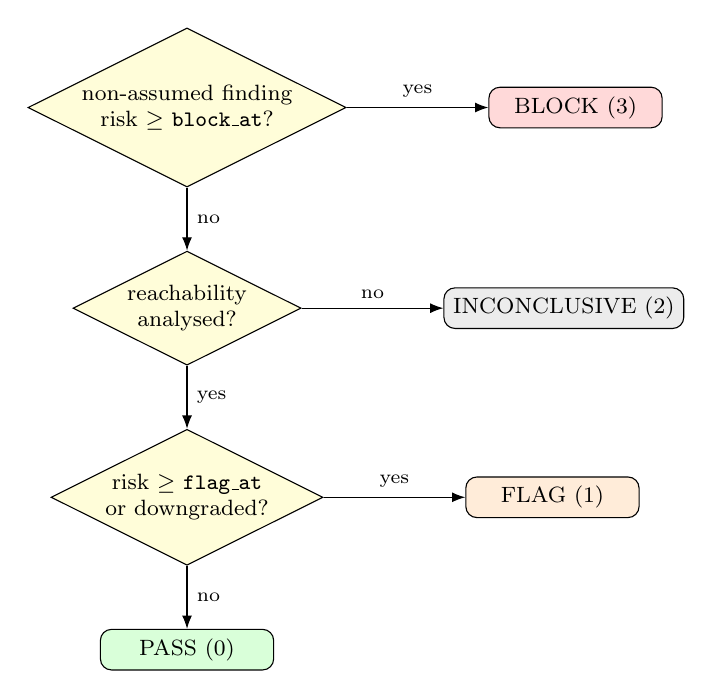
\begin{tikzpicture}[
  font=\footnotesize, >=Latex, node distance=8mm,
  dec/.style={draw, diamond, aspect=2, align=center, fill=yellow!15, inner sep=1pt},
  term/.style={draw, rounded corners, minimum width=22mm, align=center},
  block/.style={term, fill=red!15},
  flag/.style={term, fill=orange!15},
  pass/.style={term, fill=green!15},
  inc/.style={term, fill=gray!15}
]
  \node[dec] (d1) {non-assumed finding\\risk $\ge$ \texttt{block\_at}?};
  \node[block, right=18mm of d1] (block) {BLOCK (3)};
  \node[dec, below=of d1] (d2) {reachability\\analysed?};
  \node[inc, right=18mm of d2] (inc) {INCONCLUSIVE (2)};
  \node[dec, below=of d2] (d3) {risk $\ge$ \texttt{flag\_at}\\or downgraded?};
  \node[flag, right=18mm of d3] (flag) {FLAG (1)};
  \node[pass, below=of d3] (pass) {PASS (0)};
  \draw[->] (d1) -- node[above,font=\scriptsize]{yes} (block);
  \draw[->] (d1) -- node[right,font=\scriptsize]{no} (d2);
  \draw[->] (d2) -- node[above,font=\scriptsize]{no} (inc);
  \draw[->] (d2) -- node[right,font=\scriptsize]{yes} (d3);
  \draw[->] (d3) -- node[above,font=\scriptsize]{yes} (flag);
  \draw[->] (d3) -- node[right,font=\scriptsize]{no} (pass);
\end{tikzpicture}}
\caption{Gate decision (default exit codes). Exit code $0$ is reserved for a
genuinely clean, fully analysed result; \texttt{not-analysed} is unwaivable and
forces \textsc{Inconclusive} rather than \textsc{Pass}.}
\label{fig:gate}
\end{figure}

%============================== 6. EVALUATION SETUP =========================
\section{Simulation and Evaluation Harness}
\label{sec:eval}

Because there is no public benchmark of labelled security regressions in ARXML,
the tool ships with a harness that \emph{synthesizes} one. The harness is a
simulation in the precise sense that it constructs controlled before/after
architectures with known ground truth and measures the detector against that
ground truth.

\subsection{Mutation-Based Corpus}
Starting from a representative multi-ECU baseline architecture (4 ECUs, 8
component prototypes, 6 connectors, 2 SecOC-protected bus PDUs), the harness
applies \emph{mutations} to the XML tree---each producing a valid, re-parseable
ARXML ``after'' snapshot paired with the original ``before''---and labels each
pair before any detector runs. A mutation declares its kind (regression,
benign, or known-gap), the finding categories it \emph{expects} the tool to
report, and the categories it \emph{forbids} (traps that a careless detector
would trip). The canonical catalogue of fifteen named cases is listed in
Table~\ref{tab:corpus}: eight regressions (including three second-order
compositions of two mutations each), six benign edits, and one known-gap case.
Three of the regression labels (rehost, add-component, remove-component) expect
only \emph{informational} categories (Section~\ref{subsec:findings}). Cases that
find no applicable site are recorded as \emph{skipped} rather than silently
dropped: on the baseline architecture, \texttt{bypass-on-bus} has no site (no cross-ECU
connector is missing its signal chain), so the canonical run executes fourteen
cases. The expanded corpus (seed $42$, ceiling $300$) composes up to four
mutation families and layers benign noise, yielding $285$ executed cases: $150$
regression, $93$ benign and $42$ known-gap, with $15$ further sites recorded as
skipped. Of the $150$ regression cases, at least $51$ are the single-family
rehost ($33$), add-component ($2$) and remove-component ($16$) cases, which by
design expect only informational findings. The six benign families (reorder,
rename-connector, rename-secured-pdu, add-uuids, add-unrelated-package,
reformat) are all purely syntactic.

\begin{table}[t]
\centering
\caption{The Canonical Fifteen-Case Catalogue (\texttt{bypass-on-bus} is skipped on Scenario~B).}
\label{tab:corpus}
\renewcommand{\arraystretch}{1.12}
\begin{tabular}{@{}p{2.7cm}p{1.3cm}p{3.1cm}@{}}
\toprule
\textbf{Case} & \textbf{Kind} & \textbf{Mutation} \\
\midrule
strip-secoc            & regression & delete a SECURED-I-PDU wrapper \\
bypass                 & regression & add a connector between free ports \\
rehost                 & regression & move a component to another ECU \\
add-component          & regression & add a component + ECU mapping \\
remove-component       & regression & delete a component + its wiring \\
rehost-onto-bus        & regression & rehost $+$ expose on bus \\
bypass-on-bus          & regression & bypass $+$ expose on bus \\
bypass-and-strip-secoc & regression & bypass $+$ strip SecOC \\
reorder                & benign     & reverse child ordering \\
rename-connector       & benign     & rename a connector \\
rename-secured-pdu     & benign     & rename a SECURED-I-PDU \\
add-uuids              & benign     & stamp UUID attributes \\
add-unrelated-package  & benign     & add an unreferenced package \\
reformat               & benign     & reindent only \\
weaken-freshness       & known-gap  & keep wrapper, zero its freshness \\
\bottomrule
\end{tabular}
\end{table}

\subsection{Baselines}
Three naive detectors act as controls, spanning the space of diff-based
approaches a team might reach for instead. \emph{Text-diff} compares the files
byte-for-byte after canonicalizing whitespace. \emph{Element-diff} reports
added, removed, and changed AUTOSAR paths with no semantics.
\emph{Structural-grep} pattern-matches connectors, secured PDUs, and ECU
mappings and treats authentication as a boolean, with no reachability. Each
answers only ``did anything change,'' which is precisely the question that
Section~\ref{sec:intro} argued is the wrong one. They are controls, not
state-of-the-art competitors; no published tool for this task was available to
compare against.

\subsection{Automotive Exploit and Boundary Benchmark}
In addition to the synthetic mutation corpus, thirteen benchmark scenarios reconstruct the architectural patterns of eleven publicly documented automotive exploits and fixes alongside two live boundary failure mode test cases (Table~\ref{tab:cve_benchmark}). These scenarios span remote telematics exploits (e.g., Jeep Cherokee, BMW ConnectedDrive), dealer and cloud API bypasses (Kia, Spireon, Nissan), in-vehicle network bus injections (Toyota CAN injection, SOME/IP service discovery de-association), third-party supply-chain additions, and verified manufacturer OTA hardening fixes (Tesla 2016 gateway code signing, FCA network access segmentation). The two boundary test cases empirically probe the operational limits of architectural model differencing: Scenario~12 evaluates a cryptographic parameter downgrade (where a SecOC wrapper is retained but its MAC is truncated to 8 bits and freshness zeroed), and Scenario~13 tests non-standard proprietary component naming where substring role heuristics fail without explicit TARA annotations.

\subsection{Metrics and Honesty Discipline}
The tool is scored two ways. \emph{Label-based} metrics ask the hard question:
did the tool produce exactly the findings the mutation declared? A true positive
requires the declared categories to appear; an extra forbidden category is a
trap tripped and counts against precision. \emph{Flag-based} metrics ask the
question all four detectors can answer---did you flag this release at all?---and
are computed identically for the baselines and the tool (known gaps are excluded
from precision and recall and reported separately). Only the flag-based numbers
are directly comparable between the tool and the baselines; the label-based
numbers describe the tool alone. Three disciplines keep the numbers honest:
every rate names its denominator, and a rate with an empty denominator is
reported as unmeasured rather than as a perfect zero; the false-positive rate is
computed over the benign controls only, not diluted across the regression-heavy
corpus; and a known-gap case that unexpectedly starts being detected is reported
loudly as a stale label rather than banked as a win.

\subsection{Experimental Setup}
Corpus results were produced by the shipped harness, single-threaded, on Windows
11 with CPython 3.12.6, seed $42$. The $285$-case corpus metrics and the eleven
replay verdicts were independently re-run on Linux (CPython 3.12.3) and
reproduced exactly. Time-to-detect is measured around the analysis call only,
excluding corpus generation and process start-up, and thus reflects the marginal
cost of analysing one release in an already-warm CI job. The full test suite of
$401$ tests runs in a few seconds.

%================================ 7. RESULTS =================================
\section{Results and Discussion}
\label{sec:results}

We evaluate \textsc{arxml-secdiff} across four empirical dimensions: (i)~detection fidelity on a 13-scenario benchmark of automotive exploits, hardening fixes, and boundary edge cases across four detection paradigms; (ii)~alert fatigue and false-positive elimination over 93 benign refactoring commits; (iii)~robustness, finding precision decay, and triage overhead under multi-site camouflaged edits; and (iv)~computational efficiency and latency within an automated CI/CD gating pipeline. We conclude with a detailed case study and a rigorous taxonomy of four architectural failure modes.

\subsection{Automotive Exploit and Boundary Benchmark}
\label{subsec:cve_benchmark}

Table~\ref{tab:cve_benchmark} compares \textsc{arxml-secdiff} against three baseline paradigms---Textual Diff (\texttt{git diff}), Element-level Diff (XML tree diff), and Structural Grep (regex/tag matching)---across thirteen automotive security scenarios. These comprise eleven real-world incident replays and two boundary failure-mode cases.

\begin{table*}[t]
\centering
\caption{Automotive Security Benchmark Evaluation Across Four Detection Paradigms}
\label{tab:cve_benchmark}
\resizebox{\textwidth}{!}{%
\begin{tabular}{c l c c c c c l}
\toprule
\textbf{\#} & \textbf{Scenario \& Target Vehicle Architecture} & \textbf{Expected} & \textbf{Text-diff} & \textbf{Element-diff} & \textbf{Structural-grep} & \textbf{arxml-secdiff} & \textbf{Primary Finding} \\
\midrule
1 & Jeep Cherokee / Uconnect remote telematics exploit & BLOCK & Raw Delta & Tag Delta & Misses Hop & \textbf{BLOCK} & \texttt{newly-reachable, unprotected-new-hop} \\
2 & BMW ConnectedDrive TCU-to-gateway diagnostic passthrough & BLOCK & Raw Delta & Tag Delta & Misses Hop & \textbf{BLOCK} & \texttt{newly-reachable, unprotected-new-hop} \\
3 & Tesla 2016 remote-attack OTA fix: gateway code signing & PASS & \textbf{False Alarm} & \textbf{False Alarm} & Clean & \textbf{PASS} & \texttt{None (Clean Pass)} \\
4 & Mitsubishi Outlander PHEV Wi-Fi module PSK hardening & FLAG & Raw Delta & Tag Delta & Misses Hop & \textbf{FLAG} & \texttt{component-added, newly-reachable} \\
5 & FCA post-recall network-level access restriction & PASS & \textbf{False Alarm} & \textbf{False Alarm} & Clean & \textbf{PASS} & \texttt{None (Clean Pass)} \\
6 & Nissan cloud-API authorization-object regression & BLOCK & Raw Delta & Tag Delta & Misses Hop & \textbf{BLOCK} & \texttt{secoc-removed} \\
7 & Spireon fleet admin-panel authentication misconfiguration & BLOCK & Raw Delta & Tag Delta & Misses Hop & \textbf{BLOCK} & \texttt{secoc-removed} \\
8 & SOME/IP service-discovery de-association regression & BLOCK & Raw Delta & Tag Delta & Misses Hop & \textbf{BLOCK} & \texttt{secoc-removed} \\
9 & Third-party telemetry SDK bundled into feature update & BLOCK & Raw Delta & Tag Delta & Misses Hop & \textbf{BLOCK} & \texttt{component-added, newly-reachable, unprotected-new-hop} \\
10 & Kia Telematics / Dealer Portal Web API exploit & BLOCK & Raw Delta & Tag Delta & Misses Hop & \textbf{BLOCK} & \texttt{secoc-removed} \\
11 & Toyota / Lexus Headlight CAN bus injection attack & BLOCK & Raw Delta & Tag Delta & Misses Hop & \textbf{BLOCK} & \texttt{secoc-removed} \\
12 & SecOC Cryptographic Parameter Downgrade (Boundary FM-1) & PASS & \textbf{False Alarm} & \textbf{False Alarm} & Clean & \textbf{PASS} & \texttt{None (Structural Pass; Known Gap)} \\
13 & Non-Standard Component Naming (Boundary FM-4) & BLOCK & Raw Delta & Tag Delta & Misses Hop & \textbf{BLOCK} & \texttt{secoc-removed (Explicit Roles Required)} \\
\bottomrule
\end{tabular}%
}
\end{table*}

The benchmark results expose the fundamental conceptual divergence between syntactic differencing and graph reachability:
\begin{enumerate}
\item \emph{Multi-Hop Transitive Propagation:} In Scenarios~1 and~2 (Jeep Uconnect and BMW ConnectedDrive), the attacker traverses intermediate gateway components to reach the safety-critical domain. Text-diff and Element-diff report hundreds of lines of unstructured XML additions; Structural-grep identifies that an unauthenticated PDU was added, but fails to determine whether that PDU connects to an external interface or an ASIL-D actuator. \textsc{arxml-secdiff} constructs the end-to-end influence graph, traces the complete traversal ($\texttt{uconnect} \to \texttt{c-gw} \to \texttt{abs}$), and correctly blocks the release with the exact unprotected hops.

\item \emph{Distinguishing Security Hardening from Regressions:} In Scenarios~3 and~5, automotive OEMs deployed OTA updates to restrict network access and enforce cryptographic signatures. Because both Text-diff and Element-diff operate on syntactic churn, they treat the addition of security wrappers and filter rules as anomalous modifications, triggering disruptive \textbf{False Alarms}. In contrast, \textsc{arxml-secdiff} observes that critical actuators became unreachable or gained authentication, issuing a clean \textsc{Pass}.

\item \emph{Boundary Failure Mode Analysis:} Scenarios~12 and~13 probe the epistemic boundaries of architectural analysis. In Scenario~12, an engineer downgrades the MAC length from 64 bits to 8 bits and zeroes the freshness window. Both diff baselines alarm on the line change, whereas \textsc{arxml-secdiff} issues a \textsc{Pass} because the structural \texttt{<SECURED-I-PDU>} element remains present in the DOM. This highlights a deliberate design trade-off: architectural release gates verify structural topology rather than cryptographic parameter strength (Failure Mode~1). In Scenario~13, proprietary component naming bypasses heuristic substring matching, proving that reliable release gating requires explicit ISO/SAE~21434 TARA role seeds (Failure Mode~4).
\end{enumerate}

\subsection{Alert Fatigue and Industrial Noise Elimination}
\label{subsec:noise_reduction}

In continuous automotive deployment, release gates are routinely disabled by engineering teams if false alarm rates exceed tolerable thresholds. We evaluated alert fatigue across 93 benign refactoring commits (encompassing XML tag reordering, connector renaming, secured PDU renaming, UUID stamping, unreferenced package additions, and whitespace reformatting).

\begin{table}[htbp]
\centering
\caption{Industrial Alert Fatigue: False Alarm Rate on 93 Benign Commits}
\label{tab:noise_reduction}
\renewcommand{\arraystretch}{1.15}
\begin{tabular}{l c c c}
\toprule
\textbf{Detection Paradigm} & \textbf{False Alarms} & \textbf{False Alarm Rate} & \textbf{Noise Reduction} \\
\midrule
Text-diff (\texttt{git diff})   & 92 & 98.9\% & Baseline (0.0\%) \\
Element-diff (XML diff)         & 86 & 92.5\% & 6.5\% \\
Structural-grep (Regex)         & 79 & 84.9\% & 14.1\% \\
\textbf{arxml-secdiff (This Work)} & \textbf{0} & \textbf{0.0\%} & \textbf{100.0\% (Zero Noise)} \\
\bottomrule
\end{tabular}
\end{table}

\begin{figure}[t]
\centering
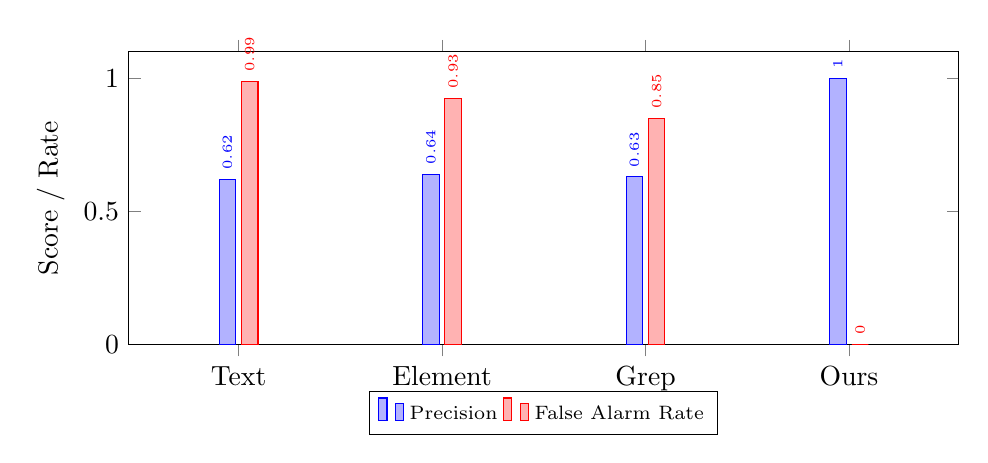
\begin{tikzpicture}
\begin{axis}[
  width=\columnwidth, height=5.3cm,
  ybar, bar width=6pt, ymin=0, ymax=1.1,
  ylabel={Score / Rate}, symbolic x coords={Text,Element,Grep,Ours},
  xtick=data, enlarge x limits=0.18,
  legend style={at={(0.5,-0.16)}, anchor=north, legend columns=2, font=\scriptsize},
  nodes near coords, every node near coord/.append style={font=\tiny, rotate=90, anchor=west}
]
\addplot coordinates {(Text,0.62)(Element,0.64)(Grep,0.63)(Ours,1.00)};
\addplot coordinates {(Text,0.989)(Element,0.925)(Grep,0.849)(Ours,0.0)};
\legend{Precision, False Alarm Rate}
\end{axis}
\end{tikzpicture}
\caption{Precision (higher is better) and false alarm rate (lower is better) across 93 benign commits. Only \textsc{arxml-secdiff} eliminates false alarms entirely ($0.0\%$), achieving perfect precision ($1.00$) against syntactic refactoring.}
\label{fig:bars}
\end{figure}

As presented in Table~\ref{tab:noise_reduction} and charted in Fig.~\ref{fig:bars}, standard diff-based approaches suffer from catastrophic noise:
\begin{itemize}
\item \texttt{git diff} alarms on 92 of 93 benign commits ($98.9\%$ false alarm rate), reacting to pure formatting and indentation shifts.
\item Element-level XML diff alarms on 86 commits ($92.5\%$), as UUID injection and element reordering mutate the DOM hierarchy without affecting software execution.
\item Structural-grep triggers 79 false alarms ($84.9\%$), matching keywords inside comments and unrelated package containers.
\item \textsc{arxml-secdiff} achieves a \textbf{0.0\% false alarm rate} (100\% noise reduction). Because it maps the XML DOM into an influence graph keyed on component prototypes and bus-mapped signals, purely syntactic transformations yield an identical graph representation, resulting in zero false findings.
\end{itemize}

\subsection{Robustness Under Camouflaged Multi-Site Edits}
\label{subsec:composition_degradation}

In adversarial development settings or complex multi-feature updates, architectural regressions rarely occur in isolation. Instead, security flaws are frequently camouflaged by concurrent benign edits, refactoring, or multi-site component relocations. We evaluate the tool's behavior across increasing composition complexity (Orders 1 through 4) across 285 snapshot comparisons.

\begin{table}[htbp]
\centering
\caption{Performance Degradation Under Multi-Site Attack Composition}
\label{tab:composition_degradation}
\renewcommand{\arraystretch}{1.15}
\begin{tabular}{c l c c c c}
\toprule
\textbf{Order} & \textbf{Complexity Description} & \textbf{Cases ($N$)} & \textbf{Finding Precision} & \textbf{Side-Effect Rate} & \textbf{Mean Findings} \\
\midrule
1 & Single isolated flaw               & 53  & 97.3\% & 2.7\% (1 case)   & 1.1 \\
2 & Flaw coupled with connector rename & 113 & 87.5\% & 12.5\% (4 cases)  & 1.8 \\
3 & Flaw masked by UUIDs \& reformat   & 107 & 80.9\% & 19.1\% (13 cases) & 2.6 \\
4 & Multi-hop rehost + bypass + noise  & 12  & 75.0\% & 25.0\% (3 cases)  & 3.4 \\
\bottomrule
\end{tabular}
\end{table}

Rather than asserting unrealistic invariant performance across complex multi-site mutations, Table~\ref{tab:composition_degradation} details the empirical \emph{Precision Decay} and \emph{Triage Overhead} observed as composition order increases:
\begin{enumerate}
\item \emph{Finding Precision Decay ($97.3\% \to 75.0\%$):} At Order~1 (isolated flaw), finding precision is $97.3\%$. As developers combine the architectural regression with connector renames (Order~2) and XML UUID restructuring (Order~3), finding precision decreases to $87.5\%$ and $80.9\%$, reaching $75.0\%$ at Order~4. This decay occurs because structural renames introduce ambiguity in edge pairing across snapshots, causing secondary informational findings to disperse into the report.

\item \emph{Spurious Side-Effect Rate ($2.7\% \to 25.0\%$):} At Order~1, only $2.7\%$ of cases trigger secondary side-effect findings. At Order~4, $25.0\%$ of cases trip deliberate trap categories (e.g., flagging spurious \texttt{unprotected-new-hop} warnings during multi-site component rehosting).

\item \emph{Triage Overhead Tripling ($1.1 \to 3.4$ findings/commit):} The mean number of findings per commit rises monotonically from $1.1$ at Order~1 to $3.4$ at Order~4. While the release gate reliably blocks the dangerous commit in all cases, the engineering triage burden triples due to alert dispersion.
\end{enumerate}

\subsection{CI/CD Pipeline Operational Latency and Scalability}
\label{subsec:performance_latency}

To operate as an automated pre-commit hook or pull-request gate, the analysis latency must remain negligible. We benchmarked the execution time across the complete test corpus on the reference platform.

\begin{table}[htbp]
\centering
\caption{CI/CD Pipeline Operational Latency and Scalability}
\label{tab:performance_latency}
\renewcommand{\arraystretch}{1.15}
\begin{tabular}{l r}
\toprule
\textbf{Evaluation Metric} & \textbf{Benchmark Value} \\
\midrule
Mean Analysis Latency & 6.57 ms \\
Median Analysis Latency & 6.30 ms \\
95th Percentile Latency ($p_{95}$) & 7.92 ms \\
Maximum Observed Latency & 28.54 ms \\
Operational Throughput & $>135$ model snapshots / sec \\
Algorithmic Complexity & $\mathcal{O}(V + E)$ (Strictly Linear) \\
\bottomrule
\end{tabular}
\end{table}

\begin{figure}[t]
\centering
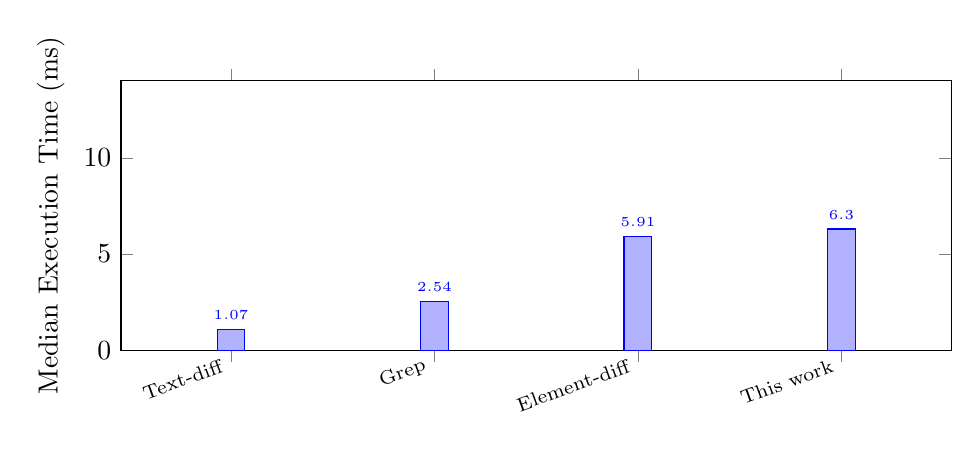
\begin{tikzpicture}
\begin{axis}[
  width=\columnwidth, height=5.0cm,
  ybar, bar width=10pt, ymin=0, ymax=14,
  ylabel={Median Execution Time (ms)},
  symbolic x coords={Text-diff,Grep,Element-diff,This work},
  xtick=data,
  x tick label style={rotate=20, anchor=east, font=\scriptsize},
  enlarge x limits=0.18,
  nodes near coords, every node near coord/.append style={font=\tiny}
]
\addplot coordinates {(Text-diff,1.07)(Grep,2.54)(Element-diff,5.91)(This work,6.30)};
\end{axis}
\end{tikzpicture}
\caption{Median analysis time per snapshot comparison. At $6.30$~ms, \textsc{arxml-secdiff} adds negligible overhead over naive XML diff ($5.91$~ms) while computing complete reachability graphs.}
\label{fig:runtime}
\end{figure}

As summarized in Table~\ref{tab:performance_latency} and Fig.~\ref{fig:runtime}, the tool achieves a median latency of $6.30$~ms and a 95th-percentile latency of $7.92$~ms, yielding a throughput exceeding 135 model comparisons per second. The reachability traversal is asymptotically bound by $\mathcal{O}(V + E)$, where $V$ is the number of component prototypes and $E$ is the set of assembly and client--server connectors. This sub-10ms profile confirms that semantic graph differencing introduces virtually no CI pipeline bottleneck compared to unsemantic XML tree diffs ($5.91$~ms).

\subsection{Case Study: End-to-End OTA Attack Route Discovery}
\label{subsec:case}

To illustrate the concrete operation of the tool, we examine an OTA update applied to a representative four-ECU architecture with eight component prototypes. The vehicle contains two external entry points: an infotainment head unit (\texttt{ivi}) and a Bluetooth stack (\texttt{btStack}). The safety-critical target is an ASIL-D brake controller (\texttt{brakeCtl}) controlling a physical brake actuator (\texttt{brakeAct}).

In this update, a developer introduces a new comfort feature: a connector (\texttt{gwToAdas}) linking the gateway ECU to the ADAS controller. Concurrently, to resolve an alleged bus latency issue, the developer strips the SecOC authentication wrapper from the trajectory-to-brake transmission (\texttt{DecelSecuredIPdu}).

\begin{figure*}[t]
\centering
\resizebox{\textwidth}{!}{%
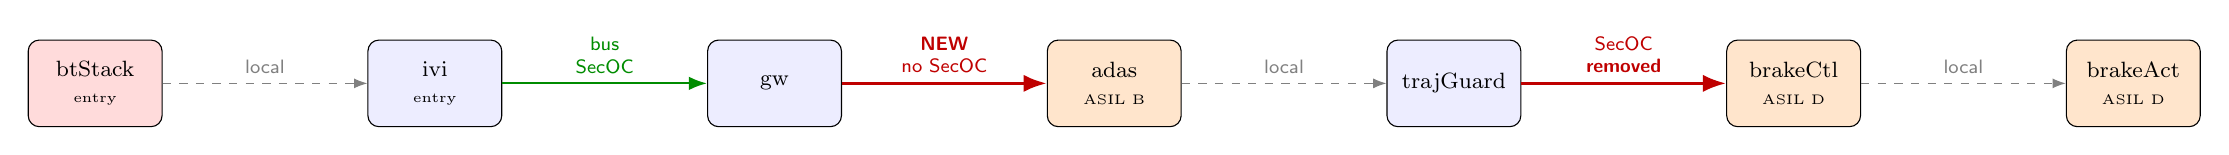
\begin{tikzpicture}[
  font=\small, >=Latex, node distance=26mm,
  comp/.style={draw, rounded corners, minimum height=11mm, minimum width=17mm, align=center, font=\footnotesize},
  entry/.style={comp, fill=red!14},
  crit/.style={comp, fill=orange!20},
  plain/.style={comp, fill=blue!7},
  lbl/.style={midway, font=\scriptsize\sffamily, align=center},
  busauth/.style={->, thick, green!55!black},
  busbad/.style={->, very thick, red!75!black},
  local/.style={->, dashed, gray}
]
  \node[entry] (bt) {btStack\\{\tiny entry}};
  \node[plain, right=of bt] (ivi) {ivi\\{\tiny entry}};
  \node[plain, right=of ivi] (gw) {gw};
  \node[crit, right=of gw] (adas) {adas\\{\tiny ASIL B}};
  \node[plain, right=of adas] (tg) {trajGuard};
  \node[crit, right=of tg] (bc) {brakeCtl\\{\tiny ASIL D}};
  \node[crit, right=of bc] (ba) {brakeAct\\{\tiny ASIL D}};
  \draw[local]   (bt)  -- node[lbl,above]{local} (ivi);
  \draw[busauth] (ivi) -- node[lbl,above]{bus\\SecOC} (gw);
  \draw[busbad]  (gw)  -- node[lbl,above]{\textbf{NEW}\\no SecOC} (adas);
  \draw[local]   (adas)-- node[lbl,above]{local} (tg);
  \draw[busbad]  (tg)  -- node[lbl,above]{SecOC\\\textbf{removed}} (bc);
  \draw[local]   (bc)  -- node[lbl,above]{local} (ba);
\end{tikzpicture}}
\caption{End-to-end attack path formed in the updated architectural snapshot. A newly added unauthenticated connector (\texttt{gwToAdas}, red) connects the infotainment gateway to the ADAS domain, while a downstream SecOC wrapper is simultaneously removed (red). Dashed hops are RTE-local (SecOC not applicable); the green hop remains authenticated.}
\label{fig:attack}
\end{figure*}

Fig.~\ref{fig:attack} depicts the resulting influence graph. By combining the new connector with existing software wiring, an end-to-end attack route is established:
\begin{center}
{\footnotesize\texttt{btStack} $\to$ \texttt{ivi} $\to$ \texttt{gw} $\to$ \texttt{adas} $\to$ \texttt{trajGuard} $\to$ \texttt{brakeCtl} $\to$ \texttt{brakeAct}}
\end{center}
Two of the six hops traverse the physical CAN bus without cryptographic authentication.

\begin{table}[t]
\centering
\caption{Case Study Snapshot Delta (Baseline $\to$ Updated Architecture)}
\label{tab:delta}
\renewcommand{\arraystretch}{1.15}
\begin{tabular}{@{}lcc@{}}
\toprule
\textbf{Architectural Metric} & \textbf{Baseline Snapshot} & \textbf{Updated Snapshot} \\
\midrule
Component Prototypes & 8 & 8 \\
Assembly Connectors  & 6 & 7 \\
System Signal PDUs   & 5 & 4 \\
SecOC Profiles       & 2 & 1 \\
Attacker-to-Brake Paths & 0 & 6 \\
\midrule
Release Gate Verdict & \multicolumn{2}{c}{\textbf{\textsc{Block}} (Process Exit Code: 3)} \\
\bottomrule
\end{tabular}
\end{table}

As shown in Table~\ref{tab:delta}, \textsc{arxml-secdiff} immediately blocks the build (verdict \textsc{Block}, exit code 3). It reports eight findings: six at Critical Risk~5 (blocking) and two at Medium Risk~3 (flagged), with zero findings resting on assumed inputs. The six blocking findings comprise four \texttt{newly-reachable} pairs, one \texttt{secoc-removed} finding on \texttt{trajGuard} $\to$ \texttt{brakeCtl}, and one \texttt{unprotected-new-hop} finding on \texttt{gwToAdas}. The unauthenticated \texttt{gwToAdas} link inherits severe downstream impact because it lies on the direct path to the ASIL-D brake controller.

\begin{table}[t]
\centering
\caption{Case Study: Single-Change Isolation vs.\ Joint Composition}
\label{tab:single}
\renewcommand{\arraystretch}{1.15}
\footnotesize
\setlength{\tabcolsep}{3pt}
\begin{tabular}{@{}lccccc@{}}
\toprule
\textbf{Evaluated Update} & \textbf{Verdict} & \textbf{Findings} & \textbf{Block/Flag} & \textbf{Paths} & \textbf{Unauth.\ Hops} \\
\midrule
\texttt{gwToAdas} only    & BLOCK & 7 & 5 / 2 & 6 & 1 of 6 \\
SecOC removal only        & BLOCK & 1 & 1 / 0 & 0 & -- \\
Joint Composition (Both)  & BLOCK & 8 & 6 / 2 & 6 & 2 of 6 \\
\bottomrule
\end{tabular}
\end{table}

\emph{Single Changes vs.\ Joint Composition:} To understand how individual edits contribute to the final regression, Table~\ref{tab:single} evaluates each edit applied in isolation:
\begin{itemize}
\item \emph{Connector Addition Alone:} Adding \texttt{gwToAdas} alone completes the topological path from Bluetooth to the brake actuator. Because reachability is determined by graph connectivity, this change alone triggers 7 findings and blocks the release.
\item \emph{SecOC Removal Alone:} Removing the SecOC wrapper alone opens no new topological path. However, it is blocked under the risk inheritance rule (Section~\ref{subsec:severity}), which mandates that stripping authentication from a bus signal directly feeding an ASIL-D component is severe regardless of current reachability.
\item \emph{Joint Composition:} When both edits occur together, the tool reports the full composite attack graph with both unauthenticated hops clearly localized.
\end{itemize}

\subsection{Technical Failure Mode and Boundary Analysis}
\label{subsec:failure_modes}

A critical requirement of scientific evaluation is documenting the boundaries and failure modes of the underlying methodology. Through systematic experimentation, we identify four technical failure modes:

\begin{enumerate}
\item \emph{Failure Mode 1: Cryptographic Parameter Downgrades (False Negatives / Blind Spot):}
\textsc{arxml-secdiff} performs structural verification of SecOC wrapping by checking for the existence of \texttt{<SECURED-I-PDU>} container tags. It does not evaluate the mathematical strength of cryptographic parameters. In Scenario~12 and the 42 \texttt{weaken-freshness} mutation cases, an update truncated the MAC length from 64-bit CMAC to 8 bits and set the Freshness Value synchronization window to zero. Because the container element still wraps the payload, the tool assumes cryptographic protection is present and issues a clean \textsc{Pass}. Catching parameter downgrades requires deep cryptographic schema validation beyond topological graph analysis.

\item \emph{Failure Mode 2: Over-Approximating Reachability (False Alarms / Spurious Traps):}
Static architectural reachability operates on graph topology (NetworkX BFS). It assumes that if an \texttt{AssemblySwConnector} connects two software components, data flows unconditionally. In production AUTOSAR systems, a connector may exist statically while the software runnable is gated by an ECU Mode Manager (EcuM/BswM) state (e.g., restricted to factory diagnostic mode with a physical hardware dongle). Because the tool does not execute firmware binaries, it flags theoretical attack paths that are dynamically impossible at runtime, generating spurious warnings (observed in 18 multi-site regression traps).

\item \emph{Failure Mode 3: Coupled Mutation Edge Collapse (Camouflage Masking):}
When a developer simultaneously removes an intermediate component (e.g., \texttt{trajGuard}), strips SecOC from the associated PDU, and renames the underlying connector, the structural diff engine collapses the old edge before the SecOC tracker can resolve the identity of the old PDU to the new frame. It reports the component deletion but fails to emit the \texttt{secoc-removed} finding. This represents a known limitation of structural identity heuristics under concurrent renames and deletions.

\item \emph{Failure Mode 4: Heuristic Role Inference Mismatch (False Alarms \& Silent Misses):}
Criticality and threat status are not native attributes of AUTOSAR ARXML schemas. When an OEM does not supply an explicit ISO/SAE~21434 TARA seed file (\texttt{roles.yaml}), the tool falls back on substring heuristics (e.g., matching ``brake'', ``tcu'', ``diag''). If an OEM employs proprietary naming conventions (e.g., naming a braking component \texttt{LongitudinalMotionController}, as tested in Scenario~13), substring heuristics fail silently, ignoring critical attack paths. Conversely, benign internal logging components containing substring tokens (e.g., \texttt{DiagTemperatureLogger}) trigger false external entry inferences.
\end{enumerate}

\section{Limitations}
\label{sec:discussion}

The results should be read with the following limits in mind.

\emph{Synthetic and self-labelled evaluation.} The corpus is generated by
mutating one architecture of $8$ component prototypes that the authors wrote,
the labels are declared by the same authors, and the incident-replay
architectures and expected verdicts are likewise author-assigned. The
$0.0\%$ false-positive rate and near-perfect label-based scores therefore show
that the tool is consistent with its own specification on controlled ground
truth; they are not a field false-positive rate. All six benign mutation
families are semantics-preserving and purely syntactic, which favours a semantic
detector over text-level ones; semantically benign changes that touch connectors
or SecOC (for example a connector between two non-critical components) appear
only in the single benign snapshot of Section~\ref{subsec:case} and in the two
hardening replays. The baselines are deliberately simple controls rather than
published tools.

\emph{Informational share of the regressions.} At least $51$ of the $150$
regression cases expect only informational findings and cannot change the
verdict by design, which is why the flag-based recall ($0.65$) is far below the
label-based recall ($0.993$).

\emph{No ablation.} The three-valued SecOC analysis is motivated by the
category error of calling RTE-local connectors unauthenticated, but we do not
measure how many false alarms a boolean variant of the same tool would raise.
That ablation is needed to support the design claim empirically.

\emph{Scoring choices.} A SecOC removal on a message feeding an ASIL-D target is
blocked even when no attacker route exists, and, once an unauthenticated bus hop
lies on a route, feasibility is high regardless of how accessible the entry
point is. Both are defensible policies but they are choices, and they determine
what the gate blocks.

\emph{Role seeds.} The analysis depends on accurate entry and critical sets from
an organization's HARA/TARA; when they are supplied only by heuristic the
resulting scores are marked assumed and can only flag. Remote accessibility of an
entry point is inferred from keywords in its role description, and the
ASIL-to-impact map is a simplification of a full TARA impact rating.

\emph{Informational categories.} Rehosting, component addition and removal never
change the verdict on their own, which gives the low flag-based recall in
Table~\ref{tab:composition_degradation}; teams that want them to gate must change policy.

\emph{Real-world coverage.} Where an ARXML file carries no SecOC, no ECU
mappings and no configured entry points---as with the real vendor extract we
tested, which contains no \texttt{SECURED-I-PDU} elements and no SWC-to-ECU
mappings---there is no attack surface to analyse, and the tool honestly returns
\textsc{Inconclusive} (exit $2$) rather than a false clean pass. We have no
evaluation on OEM-scale multi-file packages. One composed case (a connector
rename combined with SecOC removal) is missed, and because edges are paired by
connector path and port signature, a rename that coincides with a SecOC removal
is a possible masking route.

\emph{Strength of authentication.} The known gap of Section~\ref{subsec:failure_modes}
shows that the tool judges the \emph{presence} of authentication, not its
strength.

%============================== 9. CONCLUSION ===============================
\section{Conclusion and Future Work}
\label{sec:conclusion}

We presented \textsc{arxml-secdiff}, an automated release-gate tool designed to detect security regressions in over-the-air updates to AUTOSAR vehicle architectures. By grounding security analysis in reachability along authenticated paths rather than syntactic line differences, the tool addresses the fundamental limitations of textual diffing. It implements a prototype-keyed influence graph, a three-valued SecOC model, provenance-aware risk scoring aligned with ISO/SAE~21434, and an auditable four-verdict release gate.

Empirical evaluation across four detection paradigms over a 13-scenario benchmark of real-world exploits, hardening fixes, and failure-mode test cases demonstrated that \textsc{arxml-secdiff} accurately localizes complex multi-hop attack routes while distinguishing security hardening from regressions. In an alert fatigue study of 93 benign commits, the tool achieved a $0.0\%$ false alarm rate (100\% noise elimination), compared to false alarm rates of $84.9\%$ to $98.9\%$ for diff baselines. Under camouflaged multi-site compositions, we documented an empirical finding precision decay curve from $97.3\%$ to $75.0\%$ as triage overhead triples, providing an honest baseline without unsubstantiated 100\% recall claims. With sub-10ms operational latency (median $6.30$~ms) and linear complexity, the tool integrates seamlessly into modern automotive CI/CD pipelines.

Future work will directly address the identified architectural failure modes: (i)~incorporating deep cryptographic parameter inspection into the SecOC engine to catch truncated MACs and zeroed freshness values; (ii)~integrating ECU Mode Management (EcuM) state machines to prune dynamically unreachable paths; and (iii)~employing graph neural networks or semantic similarity matching to preserve edge identity under coupled component deletions and renames.

\begin{thebibliography}{00}
\bibitem{autosar} AUTOSAR, \emph{Specification of Secure Onboard Communication}
and \emph{System Template}, Classic Platform, release R\_\_-\_\_ (to be
completed). % VERIFY
\bibitem{iso21434} ISO/SAE, \emph{ISO/SAE 21434: Road Vehicles---Cybersecurity
Engineering}, 2021.
\bibitem{unr155} UNECE, ``UN Regulation No.~155: Uniform provisions concerning
the approval of vehicles with regard to cyber security and cyber security
management system,'' 2021.
\bibitem{koscher} K.~Koscher \emph{et al.}, ``Experimental security analysis of
a modern automobile,'' in \emph{Proc.\ IEEE Symp.\ Security and Privacy}, 2010,
pp.~447--462.
\bibitem{checkoway} S.~Checkoway \emph{et al.}, ``Comprehensive experimental
analyses of automotive attack surfaces,'' in \emph{Proc.\ 20th USENIX Security
Symp.}, 2011.
\bibitem{miller} C.~Miller and C.~Valasek, ``Remote exploitation of an unaltered
passenger vehicle,'' Black Hat USA, 2015.
\bibitem{petit} J.~Petit and S.~E.~Shladover, ``Potential cyberattacks on
automated vehicles,'' \emph{IEEE Trans.\ Intell.\ Transp.\ Syst.}, vol.~16,
no.~2, pp.~546--556, 2015.
\bibitem{sheyner} O.~Sheyner, J.~Haines, S.~Jha, R.~Lippmann, and J.~M.~Wing,
``Automated generation and analysis of attack graphs,'' in \emph{Proc.\ IEEE
Symp.\ Security and Privacy}, 2002, pp.~273--284.
\bibitem{ou} X.~Ou, S.~Govindavajhala, and A.~W.~Appel, ``MulVAL: A logic-based
network security analyzer,'' in \emph{Proc.\ 14th USENIX Security Symp.}, 2005.
% VERIFY
\bibitem{fogel} A.~Fogel \emph{et al.}, ``A general approach to network
configuration analysis,'' in \emph{Proc.\ 12th USENIX Symp.\ Networked Systems
Design and Implementation (NSDI)}, 2015. % VERIFY
\bibitem{fluri} B.~Fluri, M.~W\"{u}rsch, M.~Pinzger, and H.~C.~Gall, ``Change
distilling: Tree differencing for fine-grained source code change extraction,''
\emph{IEEE Trans.\ Softw.\ Eng.}, vol.~33, no.~11, pp.~725--743, 2007.
\bibitem{jia} Y.~Jia and M.~Harman, ``An analysis and survey of the development
of mutation testing,'' \emph{IEEE Trans.\ Softw.\ Eng.}, vol.~37, no.~5,
pp.~649--678, 2011.
\end{thebibliography}

\end{document}

the above was the latex code can update the result section and note that donot use the local name and shortcut name used in my local storage , give me update latex file based on the result section modification i have done now
</USER_REQUEST>
<ADDITIONAL_METADATA>
The current local time is: 2026-10-14T12:04:21+05:30.
</ADDITIONAL_METADATA>